\chapter{Basistechnologien}
\thispagestyle{standard}
\pagestyle{standard}
\renewcommand{\footrulewidth}{0.4pt}
\lfoot{\small Refik Kerimi}

\section{Aufbau PWA}
IN diesem Kapitel werden die Vorteile/Nachteile im Vergleich zu den \acl{NA}s aufgelistet und der Aufbau einer \acs{PWA} erklärt.  

  \begin{figure}[h]
	\centering
	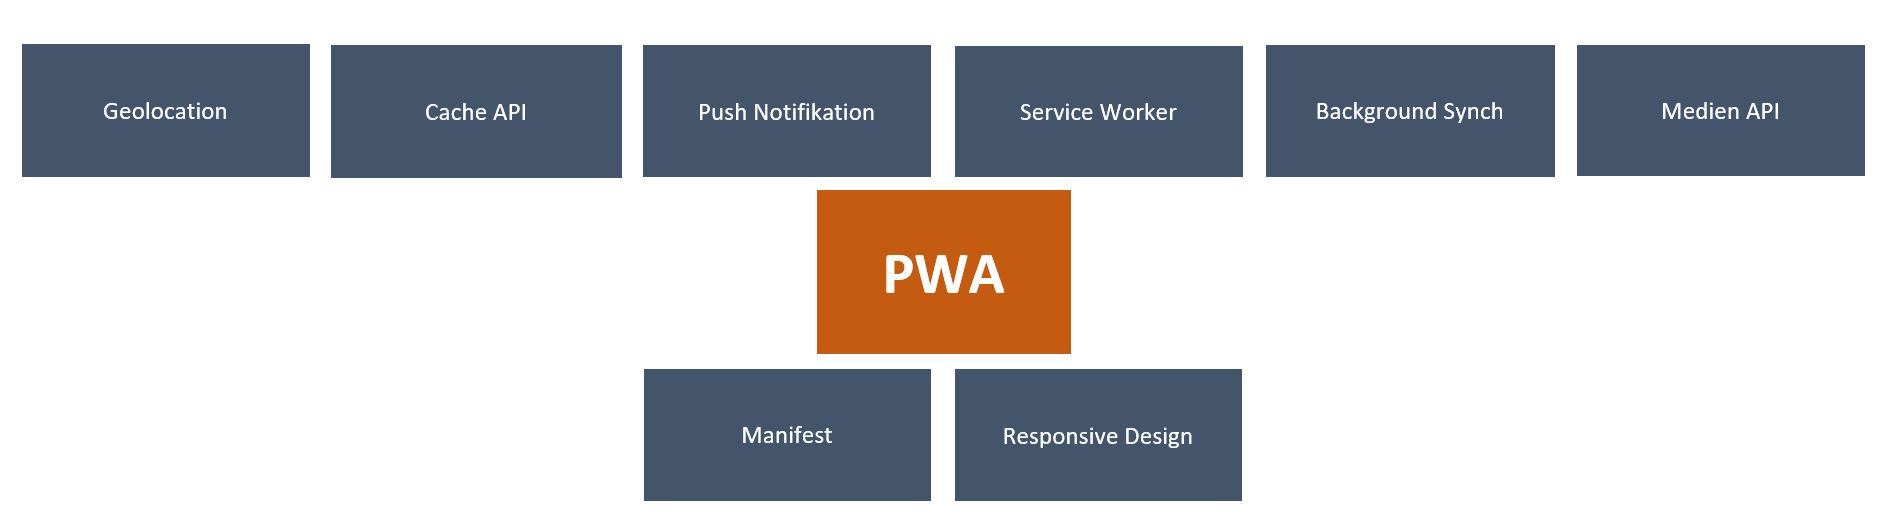
\includegraphics[width=14cm]{BilderAllgemein/PWA_Features}\medskip
	\caption{PWA Komponenten}
	\label{fig:Komponenten}
\end{figure}

\subsection{Tabelle}


%Tabelle verwenden





\section{Web App Manifest}
Das App Manifest ist ein JSON File verrät dem Browser wie sich die \acs{WA}, bei der Installation auf dem Startbildschirm, verhält. Im Manifest wird der Name,der Kurzname, die Größe, Aussehen der Icons und weitere Eigenschaften definiert diese im Kapitel \ref{chap:Entwurf} näher erklärt werden.

\subsection{Bereitstellung des Web App Manifest}
das App Manifest.json file wird in die gleiche Ebene wie die Index.html Datei in das Projekt eingepflegt und und übre den folgenden Link-Tag in der Index Datei bereitgestellt:


\begin{lstlisting}[language=HTML, caption={Manifest.json},label=lst:Manifest.json, xleftmargin=50pt]
<link rel="manifest" href="/<Dateinname>">
\end{lstlisting}

Der Aufbau der Manifest ist wie in Listening (Nr) gezeigt aufgebaut:







\cite{Manifest}


\section{Service Worker}
%\label{sec:Service Worker} zuweisung zu anderen Sektor
Der \acl{SW} (\acs{SW}) ist ein Script das der Browser im Hintergrund ausführt \cite{RegistrierungServiceWorker}. Mit der Hilfe des \acs{SW} ist es möglich die \acs{WA} offline zu betreiben, Push Notifikation zu erhalten, gecachte Daten abzurufen. \acs{SW} verhalten sich wie Proxy-Server, welche in einer Zwischenschicht vom Browser und den Netzwerk sitzen. 
Ein \acs{SW} wird von einem Worker-Kontext \cite{Worker} ausgeführt, hat keinen DOM Zugriff und wird als Haupt-Java Script Thread verwendet \cite{ServiceWorker}.

\subsection{Basis Architektur}
Der Cyclus eines \acs{SW}s ist von der Webseite getrennt.
In der Installationsphase werden benötigte statische Datein zwischengespeichert erst danach ist der \acs{SW} installiert. Die Installation erfolgt über die JavaScript-Funktion:

\begin{lstlisting}[language=JavaScript, caption={Service Worker Navigator},label=lst:ServiceWorkerNavigator, xleftmargin=50pt]
navigator.serviceWorker.register
\end{lstlisting}

Danach folgt die Aktivierungsphase, in dieser Phase werden alte Cache-Inhalte verwaltet und Aktualisiert.


\begin{figure}[h]
	\centering
	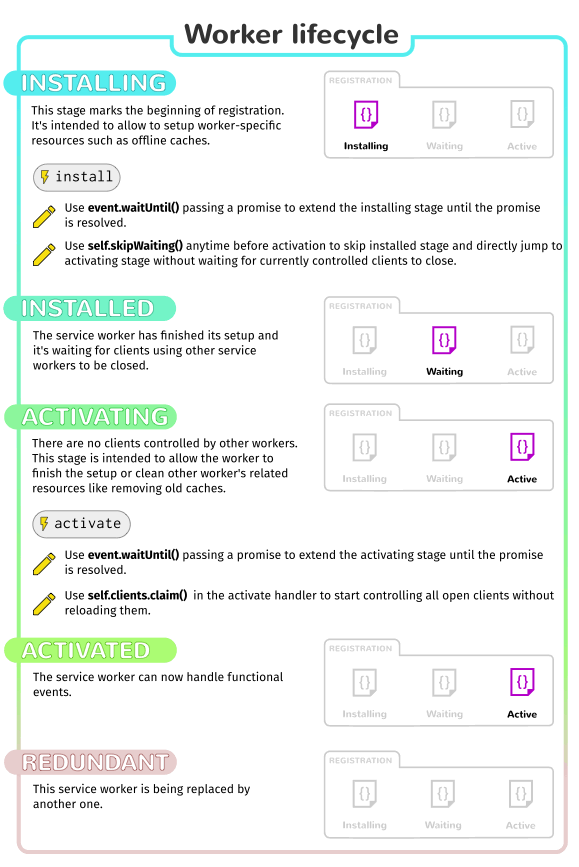
\includegraphics[width=8cm]{BilderAllgemein/swLifecycle}\medskip
	\caption{Basis Architektur \acl{SW}}
	\label{fig:Erstinstallation}\cite{ServiceWorkerArchitecture}
\end{figure}
Um die neuen Seiten zu steuern muss der \acs{SW} erneut geladen werden.
In der Abbildung \ref{fig:Erstinstallation} ist eine vereinfachte Erstinstallation zu sehen:

\subsection{Registrierung Service Worker}

Um den \acs{SW} zu registrieren muss folgender \acs{JS}-Code in das Projekt im (genauen Pfad rausfinden) integriert werden.
\begin{lstlisting}[language=JavaScript, caption={Service Worker Register},label=lst:ServiceWorkerRegister, xleftmargin=50pt]
if ('serviceWorker' in navigator) {
  window.addEventListener('load', function() {
    navigator.serviceWorker.register('/sw.js').then(function(registration) {
      // Registration was successful
      console.log('ServiceWorker registration successful with scope: ', registration.scope);
    }, function(err) {
      // registration failed :(
      console.log('ServiceWorker registration failed: ', err);
    });
  });
}
\end{lstlisting}

Hier wird die Unterstützung durch den Browser geprüft.

\begin{figure}[h]
	\centering
	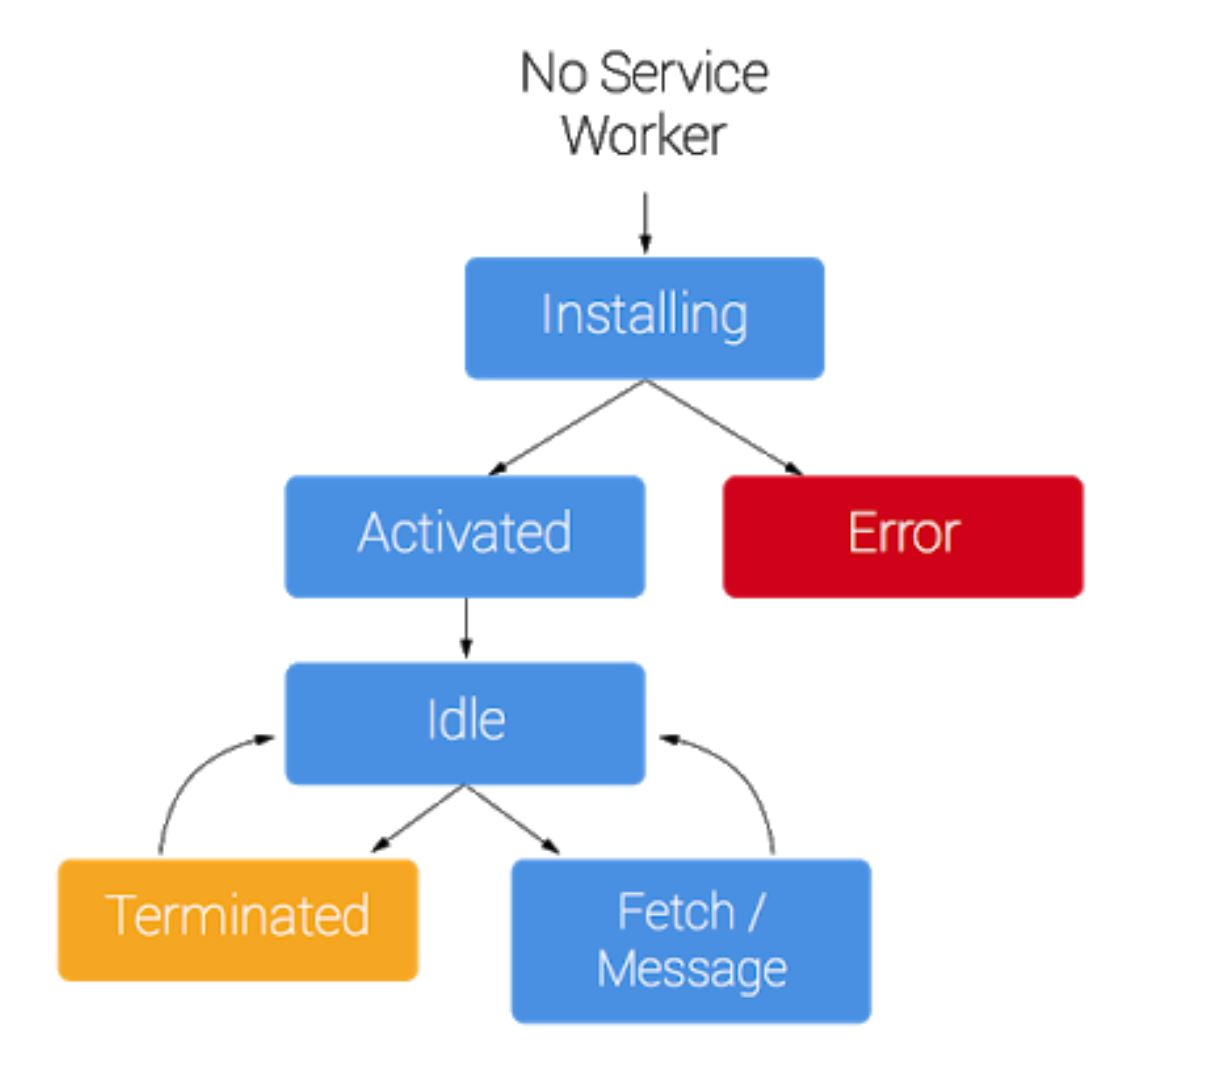
\includegraphics[width=14cm]{BilderAllgemein/InstallSW}\medskip
	\caption{Erstinstallation Service Worker}
	\label{fig:Erstinstallation}\cite{ServiceWorkerRegistration}
\end{figure}

Der \acs{SW} kann nach der Übernahme der Steuerung zwei Zustände übernehmen, entweder dieser wird beendet oder er übernimmt die Verwaltung der Netzwerkanfragen und der Nachrichten \cite{ServiceWorkerRegistration}.

\newpage

\section{Push Notifikation}
Um dem User bei einer \acs{PWA} das Gefühl einer Native App aufkommen zu lassen ist die Push Funktion unablässig. Erst durch diese Funktion in Kombination mit dem \acs{SW} gibt der \acl{WA} die persönliche Nähe zum User \cite{PushNotifikation}.


\subsection{Registrierung Push Notifikation}
Um die Push Funktion zu integrieren muss die Registerfunktion des \acs{SW} wie folgt erweitert werden:
 
\begin{lstlisting}[language=JavaScript, caption={Push Notifications},label=lst:PushNotifikation, xleftmargin=50pt]

if ('serviceWorker' in navigator && 'PushManager' in window) {
  console.log('Service Worker and Push is supported');

  navigator.serviceWorker.register('sw.js')
  .then(function(swReg) {
    console.log('Service Worker is registered', swReg);

    swRegistration = swReg;
  })
  .catch(function(error) {
    console.error('Service Worker Error', error);
  });
} else {
  console.warn('Push messaging is not supported');
  pushButton.textContent = 'Push Not Supported';
}
\end{lstlisting}


Hier wird der Support der Pushfunktionen durch den Browser überprüft wie in Kapitel \ref{chap:RegistrierungServiceWorker} die Browserunterstützung vom\acs{SW} und die Push Benachrichtigung. Bei fehlerlosen Durchlauf wird die \acs{SW}.js Datei registriert \cite{PushNotifikation}.

\newpage
\subsection{Cache API}

\subsection{Geolocation}
https://appdevelopermagazine.com/5877/2018/3/1/progressive-web-apps-vs-native-apps:-showdown-in-2018/


\subsection{Camera API}


\subsection{Browser} 

